

\chapter{Fundamentos Teóricos}

En este capítulo se expone el marco contextual de las herramientas sobre las que se desarrolla esta tesis, cobrando especial importancia para comprender la metodología de este estudio en su totalidad. Es por esto por lo que en este apartado se introducen conceptos y métodos que se referencian a lo largo de todo el documento. Las siguientes secciones definen cada una de las herramientas utilizadas en este trabajo.


%\section{Modelos estado del arte}
\section{Modelos utilizados en la comparativa}

%\textcolor{blue}{\textbf{Luis: No me termina de convencer, tengo que darle otra vuelta. Me da la sensación de que se explican las fórmulas y ya, no se interpretan. Lo dejo para más adelante sabiendo esto.}}

%\underline{Modelos del estado del arte contra los que nos comparamos.}

En el campo de la inteligencia artificial y, más concretamente, el aprendizaje automático, muchos han sido los modelos y los métodos que se han desarrollado a lo largo de la historia reciente. Parte de ellos han tenido una gran relevancia debido a que han sido ampliamente aplicados en distintos tipos de problemas ofreciendo gran calidad en sus resultados, llegando a una gran capacidad de generalización en distintos contextos. Por este motivo, en este trabajo se tomarán como referencia algunos de estos métodos para la realización de una comparativa de eficiencia a través de distintas métricas. En esta sección, se describen a nivel teórico los modelos de Aprendizaje Automático que son relevantes para la comprensión y desarrollo de esta tesis. 


\subsubsection*{Gaussian Naive Bayes (GNB)}


El algoritmo \textit{Naive Bayes} es un método de Aprendizaje Supervisado ampliamente extendido en problemas de clasificación de datos, tanto por su simplicidad como por la capacidad de generalización en la calidad de los resultados que este ofrece en numerosos problemas de clasificación. Por ejemplo, este algoritmo ha sido aplicado en investigaciones recientes en detección de enfermedades cardiovasculares \cite{Sai_Krishna_Reddy_2022}, detección de ciberataques en redes inalámbricas \cite{9817298} o reconocimiento de escenas a través de imágenes mediante características geométricas presentes en ellas \cite{rafique2019scene}. La denominación de este modelo se debe a que su funcionamiento está basado el teorema de Bayes, ya que este algoritmo calcula la probabilidad de pertenencia de una muestra en base a la suposición de que cada una de las variables (predictoras) presenta una independencia condicional respecto al resto de ellas. Una de las variantes de este algoritmo para trabajar con variables numéricas es el \textit{Gaussian Naive Bayes (GNB)}. Este algoritmo trabaja con las probabilidades a priori de pertenencia de las muestras a una determinada clase, calculada sin tener en cuenta las variables predictoras de los datos, junto con las probabilidades a posteriori, aquellas individuales de cada característica una vez se toma conocimiento de los datos de entrenamiento, siendo la predicción final de este algoritmo una combinación de la composición de ambas.

La fórmula que representa la probabilidad a priori $P(y)$ de una clase $y$ viene representada por la siguiente fórmula:\\

\[
P(y) = \frac{\text{Número de muestras de la clase } y}{\text{Número total de muestras}}
\]

%Por otra parte, cada una de las variables de los datos de entrenamiento son proyectadas en distribuciones gaussianas, para cada una de las clases a predecir siguiendo la siguiente fórmula:

%\textbf{Luis: buscar las fórmulas a posteriori}

En tiempo de inferencia, la predicción de una nueva muestra se interpreta como aquella probabilidad más alta en base a las clases, haciendo uso de la información que ha obtenido el modelo en base a sus datos de entrenamiento. En la Figura \ref{GNB_BACKGROUND} se puede observar un ejemplo de distribución de datos en base al algoritmo \textit{Gaussian Naive Bayes} \cite{GNBIMAGE}.


\begin{figure}[H]
	\centering
	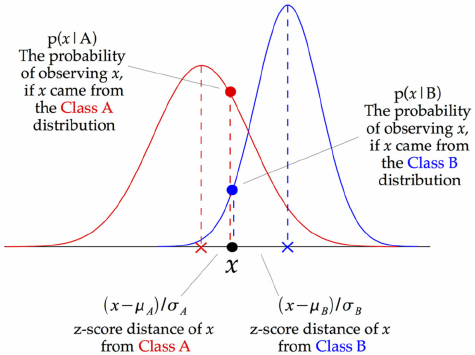
\includegraphics[width=8cm]{Figures/Background/GNB.png}
	\caption{Ejemplo de distribuciones en base a \textit{Gaussian Naive Bayes}}
	\label{GNB_BACKGROUND}
\end{figure}


\subsubsection*{Multi Layer Perceptron (MLP)}

%\textcolor{purple}{\textbf{Jose:} faltaría poner un par de referencias modernas.}

%\textbf{Luis: si explico el MLP en detalle, entraría en conflicto con la siguiente sección de modelos CNN, tendria que explicar de nuevo el Bakpropagation, gradientes, etc..}

%\textcolor{orange}{\textbf{Luis: } Hecho}

El Perceptrón Multicapa o \textit{Multi-Layer Perceptron (MLP)} es una arquitectura de red neuronal artificial. Es una generalización del Perceptrón simple y surgió como consecuencia de las limitaciones de dicha arquitectura en lo referente al problema de la separabilidad no lineal. El MLP es un aproximador universal, en el sentido de que cualquier función continua en un espacio $R^n$ puede aproximarse con un Perceptrón multicapa, con al menos una capa oculta de neuronas. Esto, sitúa al MLP como un modelo matemático útil a la hora de aproximar o interpolar relaciones no lineales entre datos de entrada y salida.

La arquitectura de Perceptrón multicapa se caracteriza porque tiene sus neuronas agrupadas en capas de diferentes niveles: la capa de entrada, las capas ocultas y la capa de salida. Las neuronas de la capa de entrada se encargan únicamente de recibir las señales del exterior y propagarlas a todas las neuronas de la siguiente capa. La última capa proporciona la respuesta de la red para cada uno de los patrones de entrada.

Este tipo de arquitecturas son ampliamente utilizadas en problemas de aprendizaje supervisado, como clasificación y regresión, y ofrecen un gran rendimiento en contextos muy variables. Por ejemplo, en publicaciones recientes, este tipo de modelos ha sido aplicado a problemas como segmentación de imágenes médicas para la prevención de múltiples enfermedades \cite{valanarasu2022unext}, para la clasificación de nubes de puntos en tres dimensiones \cite{choe2022pointmixer} o como apoyo para la predicción del tiempo estimado de trayectos en taxi de la ciudad de Nueva York \cite{poongodi2022new}. Al pertenecer a la familia de las redes neuronales, estos modelos aprenden los pesos asignados a cada una de las conexiones entre neuronas de las capas para dar lugar a las fases comunes de optimización de redes neuronales que detallarán en la sección \ref{CNN_SECTION}. En la Figura \ref{MLP_BACKGROUND} se puede observar un ejemplo de la arquitectura \textit{MLP} \cite{PEDRO2017111}.

\begin{figure}[H]
	\centering
	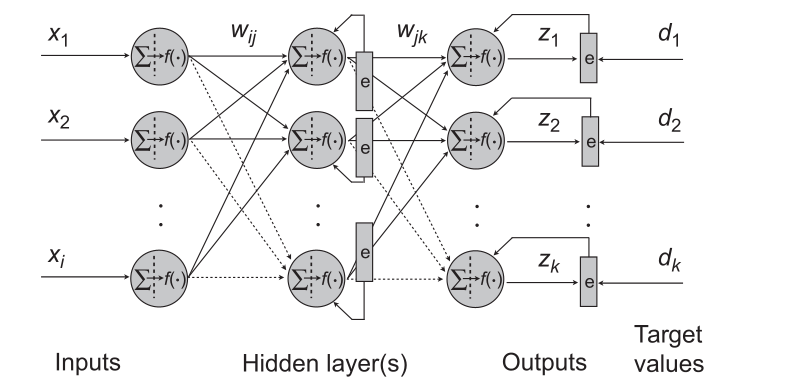
\includegraphics[width=10cm]{Figures/Background/MLP.png}
	\caption{Ejemplo de arquitectura \textit{MLP}}
	\label{MLP_BACKGROUND}
\end{figure}


% \begin{itemize}
	%     \item $x = (x_1, x_2, \ldots, x_n)$ as the input vector.
	%     \item $h^{(i)} = (h_1^{(i)}, h_2^{(i)}, \ldots, h_{m_i}^{(i)})$ as the activations of the $i$-th hidden layer.
	%     \item $W^{(i)}$ as the weight matrix connecting the $i$-th and $(i+1)$-th layers.
	%     \item $b^{(i)}$ as the bias vector added to the $i$-th layer.
	%     \item $f$ as the activation function.
	%     \item $y = (y_1, y_2, \ldots, y_k)$ as the output vector.
	% \end{itemize}

% The computation in an MLP can be represented as follows:

% \[
% h^{(i)} = f(W^{(i)}h^{(i-1)} + b^{(i)})
% \]

% where $h^{(i-1)}$ is the activation from the previous layer.

% The final output of the MLP is computed as:

% \[
% y = f(W^{(n)}h^{(n-1)} + b^{(n)})
% \]

% Here, $n$ represents the number of hidden layers in the MLP.


\subsubsection*{Regresión Logística (LR)}

%\textcolor{purple}{\textbf{Jose:} faltaría poner una imágen}

%\textcolor{orange}{\textbf{Luis: } Hecho}

La regresión logística es un modelo de aprendizaje estadístico utilizado históricamente para solventar problemas de clasificación binaria. Este método tiene como objetivo deducir la probabilidad de que ocurra un evento binario en función de uno o más predictores, siendo ampliamente extendido debido a su sencillez y capacidad de generalización. Por ejemplo, en investigaciones recientes, este modelo se ha aplicado de forma exitosa a la predicción de la pérdida de clientes en sectores de telecomunicación \cite{jain2020churn}, para la creación de rápidos protocolos computacionales de seguridad para preservar la privacidad del genoma humano \cite{de2021high}, o para la predicción de diabetes \cite{joshi2021predicting} en base a descriptores humanos. La regresión logística asigna un coeficiente a cada una de las variables predictoras, y estos son ajustados durante el proceso de aprendizaje para minimizar una función objetivo, normalmente R². Este proceso de ajuste de coeficientes en base a los datos de entrenamiento resulta en una combinación lineal de variables independientes ante nuevas muestras:

\[
z = \beta_0 + \beta_1 x_1 + \beta_2 x_2 + \dots + \beta_n x_n
\]
Donde $\beta_0, \beta_1, \dots, \beta_n$ son los coeficientes asignados a cada una de las variables predictoras, siendo $\beta_0$ el término de intercepción, y $z$ es el valor de la combinación de las características multiplicadas por dichos coeficientes.

La regresión logística hace uso de una función sigmoide, que transforma los valores continuos resultantes de la combinación lineal $z$ a una probabilidad de pertenencia a una clase en función de la separabilidad a través de esta dimensión de las muestras de entrenamiento.

\[
P(y = 1 | x) = \frac{1}{1 + e^{-z}}
\]

Donde $P(y = 1 | x)$ representa la probabilidad de la muestra x de pertenecer a la clase positiva. En la Figura \ref{LR_BACKGROUND} se puede observar un ejemplo de una clasificación mediante \textit{Regresión Logística} \cite{LR}.


\begin{figure}[h]
	\centering
	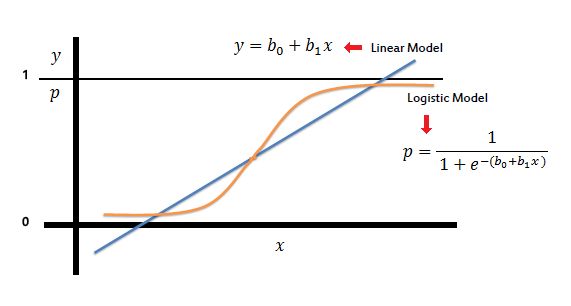
\includegraphics[width=10cm]{Figures/Background/LogReg_1.png}
	\caption{Ejemplo de clasificación mediante \textit{Regresión Logística}}
	\label{LR_BACKGROUND}
\end{figure}


\subsubsection*{k-Nearest Neighbours (KNN)}
%\textcolor{purple}{\textbf{Jose:} faltaría poner un par de referencias modernas y una imágen}
%\textcolor{orange}{\textbf{Luis: } Hecho}

El algoritmo \textit{k-Nearest Neighbours (KNN)} es un algoritmo de aprendizaje automático, ampliamente utilizado tanto para problemas de clasificación como de regresión. Estudios recientes han aplicado esta técnica para distintos propósitos, como agrupar datos de dimensiones arbitrarias para reconocer picos de densidad de forma eficiente \cite{chen2020fast}, como herramienta pra la clasificación de textos \cite{CHEN2020523}, o como apoyo para la detección de intrusos en redes inalámbricas \cite{liu2022enhanced} en base al número de usuarios por nodo, peticiones recibidas de la red, entre otras características. Este método se basa en la clasificación de nuevas muestras en base a la distancia de sus características respecto a la proyección de las muestras de entrenamiento sobre un espacio N-dimensional. Cuando una nueva muestra $x_0$ es clasificada, \textit{KNN} identifica los $K$ puntos más cercanos almacenados de sus muestras de entrenamiento respecto a las de la observación $x_0$ ($N_0$) y genera una probabilidad de pertenencia de la nueva muestra $x_0$ a la clase $j$, en función de la fracción de puntos de $N_0$ que pertenezcan a esa clase. La fórmula para calcular la probabilidad de pertenencia es la siguiente:

\[
P(y = j | X = x_0)  = \frac{1}{K} \sum_{i\in N_0} I(y_i = j)
\]

En la Figura \ref{KNN_BACKGROUND} se puede observar un ejemplo de clasificación mediante \textit{KNN} \cite{VIDUEIRAFERREIRA2015195}.

\begin{figure}[H]
	\centering
	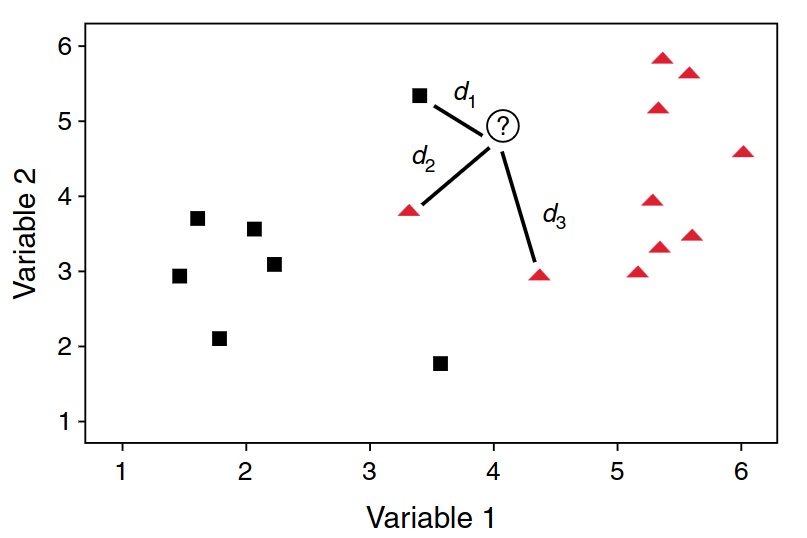
\includegraphics[width=10cm]{Figures/Background/KNN.png}
	\caption[Ejemplo de clasificación del \textit{KNN} ante una nueva muestra] {Ejemplo de clasificación del \textit{KNN} ante una nueva muestra. Se miden las distancias entre los $N$ puntos más cercanos de una nueva muestra y se clasifica como aquella que más vecinos cercanos presente}
	\label{KNN_BACKGROUND}
\end{figure}


\subsubsection*{Random Forest (RF)}
\label{RF_INTRODUCTION_TO_ENSEMBLES}

%\textcolor{purple}{\textbf{Jose:} faltaría poner un par de referencias modernas y una imágen}
%\textcolor{orange}{\textbf{Luis: } Hecho}


Los algoritmos \textit{Random Forest} son algoritmos basados en árboles de decisión que pertenecen al conjunto de modelos Ensembles. Los métodos \textit{Ensemble} son arquitecturas que están conformadas por varios modelos entrenados simultáneamente para dar lugar a un modelo predictivo final. Dentro de la categorización de Ensembles, el método \textit{Random Forest}, pertenece a la subcategoría \textit{Bagging}, cuya principal característica es que se apoyan en crear múltiples modelos que son entrenados con distintas técnicas de reemplazo (\textit{Bootstrap}) sobre los datos, conformando un modelo predictivo final como la combinación de la salida de cada uno de ellos de manera independiente por votación. Este tipo de modelos ha sido aplicado de forma efectiva en contextos muy variados, como para predicción de la contaminación de nitratos de aguas subterráneas \cite{HE2022133388}, predicción de precios de inmuebles en base a sus características \cite{ADETUNJI2022806} o para la medición de características geográficas socio-económicas importantes que influyeron en los fallecidos por \textit{COVID-19} en Estados Unidos \cite{GREKOUSIS2022102744}. Concretamente, \textit{Random Forest} se compone en $N$ árboles de decisión, donde cada uno de ellos es entrenado con un subconjunto de muestras y características de forma independiente al resto para dar lugar a un modelo combinado donde la predicción de nuevas muestras se elige aquella clase más votada de entre todo el conjunto de árboles. De forma generalizada, los modelos tipo \textit{Ensemble} son métodos robustos que son menos sensibles al sobreajuste de los datos gracias a sus técnicas de reemplazo durante su etapa de entrenamiento y la composición de un modelo final en base a varios modelos. En la Figura \ref{RF_BACKGROUND} se puede observar un ejemplo de la arquitectura \textit{Random Forest} \cite{MISRA2020243}.


\begin{figure}[H]
	\centering
	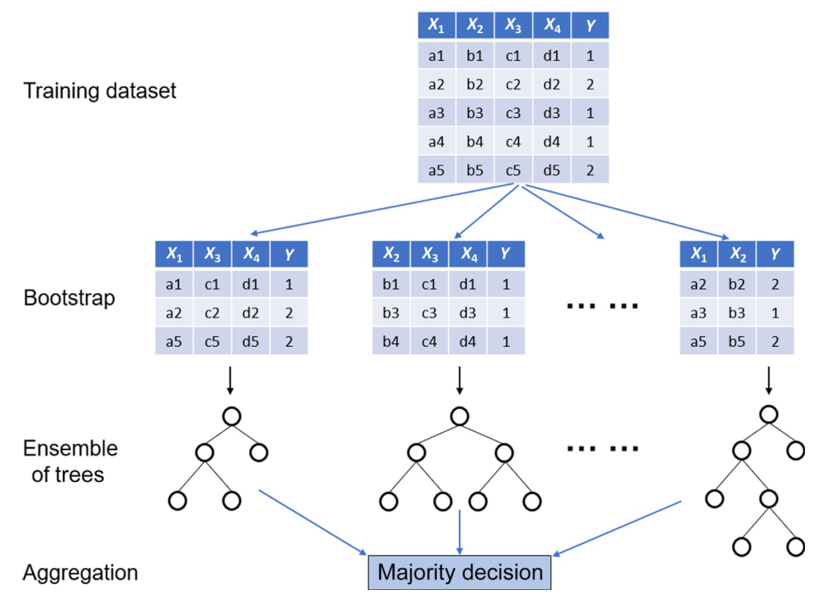
\includegraphics[width=10cm]{Figures/Background/RF.png}
	\caption[Ejemplo de arquitectura \textit{Ensemble Random Forest}]{Ejemplo de arquitectura \textit{Ensemble Random Forest}. El dataset es dividido en subconjuntos mediante \textit{Bootsrap} y se entrena un árbol de decisión sobre cada uno de ellos. La clasificación final viene dada por la predicción mayoritaria de los modelos}
	\label{RF_BACKGROUND}
\end{figure}

\subsubsection*{Support Vector Classifier (SVC)}

%\textcolor{purple}{\textbf{Jose:} faltaría poner un par de referencias modernas y una imágen}
%\textcolor{orange}{\textbf{Luis: } Hecho}

El \textit{Support Vector Classifier (SVC)} es un algoritmo de aprendizaje supervisado utilizado comúnmente para problemas de clasificación. Recientemente, este modelo ha sido aplicado a distintos contextos, como para la predicción de la deformación de los túneles durante su excavación en base a las condiciones geológicas \cite{zhou2022predicting}, como apoyo para la detección temprana de cánceres de piel \cite{arora2022bag} o incluso para la predicción de defectos en aplicaciones \textit{software} mediante métricas comunes en el desarrollo de los proyectos \cite{goyal2022effective}. Se basa en el concepto de encontrar un hiperplano óptimo que maximice la separabilidad de las clases de entrenamiento en base al espacio generado por la proyección de las características de los datos. El \textit{SVC} define estos hiperplanos en base a las muestras de distintas clases que más cerca se encuentren a lo largo del espacio N-dimensional. La fórmula que define un hiperplano para el \textit{SVC} en un problema de clasificación binario se define como:

\[
W \cdot X - b = 0
\]

En tiempo de predicción, el \textit{SVC} utiliza los hiperplanos definidos para determinar si una nueva muestra $x_0$ pertenece a una clase u otra mediante la siguiente ecuación:

\[
f({x_0}) = \text{sign}({W} \cdot {x_0} - b)
\]

Donde $W$ es el vector de pesos asociado a cada característica, $X$ es el vector de características de la muestra y $b$ es el término de sesgo.

En la Figura \ref{SVC_BACKGROUND} se puede ver un ejemplo de clasificación mediante \textit{SVC} \cite{MISRA2020243}.

\begin{figure}[H]
	\centering
	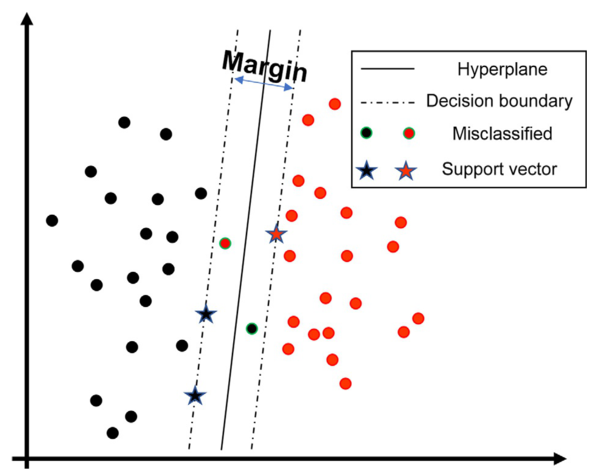
\includegraphics[width=7cm]{Figures/Background/SVC.png}
	\caption{Ejemplo de \textit{SVC}}
	\label{SVC_BACKGROUND}
\end{figure}

\section{Algoritmos CNN}
\label{CNN_SECTION}
%\underline{Explicación de diferentes algoritmos CNN con los que luego te comparas, con sus formulas y explicacion}

%\textcolor{blue}{\textbf{Luis: Yo creo que OK, hay que repasar el hilo que conecta los párrafos.}}\\


Las redes neuronales convolucionales \textit{(CNNs)} son modelos de inteligencia artificial supervisados que principalmente están orientados al reconocimiento de patrones en imágenes. Estos modelos han sido ampliamente utilizados para distintos objetivos dentro de este contexto, como clasificación de imágenes, detección de elementos de interés, o incluso han sido aplicadas a problemas de regresión. Tal es su rendimiento en estos problemas, que estas arquitecturas han sido extrapoladas al campo de la Inteligencia Artificial Generativa, ofreciendo soluciones en distintos problemas como la generación de imágenes artificiales a través de redes generativas adversarias (\textit{GANs}), segmentación de elementos de interés dentro de imágenes, o incluso en la representación de imágenes mediante vectores n-dimensionales para comparar la similitud de imágenes entre sí mediante redes siamesas.

La principal característica que distingue a estos modelos respecto al resto de redes neuronales y que las hace tan efectivas en problemas orientados a imágenes, es que su diseño se basa en capas convolucionales. Estas capas están compuestas por filtros, que durante el proceso de entrenamiento aprenden operaciones que se aplican sobre los datos de entrada, permitiendo así generar y reconocer patrones que se encuentren presentes en ellos.

Dentro de las redes neuronales convolucionales existen diferentes tipos, cada uno con sus ventajas y desventajas en función del problema que se quiera resolver. No obstante, existen partes comunes a ellas que es necesario mencionar, las capas de las que normalmente constan estas redes son las siguientes:

\begin{enumerate}
	\item \textbf{Capas convolucionales:} Estas capas aplican convoluciones sobre las muestras de entrada. Las convoluciones no son más que multiplicaciones sobre posiciones de un vector que calculan la suma ponderada de todos los vecinos de la muestra de entrada para dar lugar a un único resultado en su salida, que será asignado a la salida de la capa convolucional en la misma posición sobre la que se ha aplicado la operación sobre la muestra de entrada. Los valores de ponderación (pesos) de esta suma son aprendidos por la red en su etapa de entrenamiento.
	
	\item \textbf{Filtros:} Los filtros son pequeñas matrices de las que están compuestas las capas convolucionales y son utilizadas para realizar las operaciones. Cada uno de estos filtros tiene asociado una serie de pesos en cada posición de la matriz. Estos filtros, al ser aplicados, generan los denominados \textit{feature maps}, que no son más que mapas de activación sobre los que se aplicarán la función de activación.
	
	\item \textbf{Función de activación:} las funciones de activación de las \textit{CNN} introducen no linealidades, lo que permite a la red aprender patrones y relaciones complejas dentro de los datos. Normalmente, se aplica una función de activación como \textit{ReLU (Rectified Linear Unit)} a los mapas de características para introducir la no linealidad.
	
	\begin{center}
		$\text{ReLU}(x) = \max(0, x)$
	\end{center}
	
	\item \textbf{Capas Pooling:} estas capas aplican operaciones sobre los mapas de características con el objetivo de simplificar la información y reducir la dimensionalidad, que permite reducir la complejidad computacional de las redes durante su entrenamiento. Estas operaciones tienen una naturaleza de agrupación que son aplicadas en pequeñas zonas de los mapas de características para simplificar áreas y contemplar patrones relevantes en ellas. Estas operaciones pueden ser promediar un conjunto de características, mantener el mínimo de ellas o el máximo entre otras.
	
	\item \textbf{Capas Densas:} Las capas densas son capas que interconectan completamente un conjunto de entrada de neuronas con las neuronas especificadas en esta capa. A diferencia de su aplicación en otro tipo de redes neuronales, en las redes convolucionales estas capas toman como entrada el conjunto de características extraídas de los procesos convolucionales para dar lugar a una clasificación final.
	\begin{center}
		$z_i = \sum_{j=1}^{n} w_{ij} \cdot x_j + b_i$\\
		$y_i = f(z_i)$
	\end{center}
\end{enumerate}

%\subsubsection*{Proceso de entrenamiento de una red convolucional}

El proceso de aprendizaje de las redes neuronales está dividido en varias fases. Las redes en su etapa de entrenamiento realizan predicciones sobre los datos de entrada, aplicando operaciones matemáticas sobre ellos utilizando los pesos en cada etapa de la red, a esta etapa se le conoce como \textit{Forward Propagation}, y es definida mediante la siguiente fórmula:


\[
\mathbf{z}^{[l]} = \mathbf{W}^{[l]} \cdot \mathbf{a}^{[l-1]} + \mathbf{b}^{[l]},
\]

donde:
\begin{itemize}
	\item \(\mathbf{z}^{[l]}\) es la activación antes de aplicar la función de activación en la capa \(l\).
	\item \(\mathbf{W}^{[l]}\) es la matriz de pesos.
	\item \(\mathbf{a}^{[l-1]}\) es la salida de la capa anterior.
	\item \(\mathbf{b}^{[l]}\) es el vector de sesgo.
\end{itemize}

Posteriormente, en la capa clasificadora, los valores predichos son comparados con el valor real de las muestras que han sido introducidas en esta etapa a la red, de tal forma que el error que han producido sobre estas muestras durante esta fase es medible y calculado mediante una función de pérdida. Para llevar a cabo este proceso, es necesario introducir el concepto de función de pérdida que medirá el error durante la fase de entrenamiento


%\textbf{Función de pérdida}

Las funciones de pérdida en las redes neuronales miden el error producido por la red al realizar predicciones sobre los datos en su etapa de entrenamiento. Estas funciones tienen como objetivo comparar la calidad de la predicciones de la red respecto a la clase verdadera a la que pertenecen. Un valor alto de esta función indica un error alto en las predicciones, mientras que un valor bajo representa una buena calidad de predicciones:

\[
\text{Pérdida} = \text{Cálculo de Pérdida} (\text{Verdadero}, \text{Predicho})
\]

La función de pérdida más común en problemas de clasificación binaria es la \textit{Binary Cross Entropy} cuya fórmula es:

$$\text{Binary Cross Entropy} = \frac{-1}{N} \sum_{i=1}^{N} (y_{i}*\log{p_{i}}+ (1 - y_{i})*\log{(1-p_{i}})).$$

Con $N$ representando el número de muestras totales en el conjunto de datos, $y_i$ la etiqueta verdadera de la clase (0 ó 1) de la muestra actual y $p_i$ la probabilidad de que la muestra actual pertenezca a la clase $1$.

Esta ecuación penaliza en tiempo de entrenamiento la clasificación errónea de las muestras. El término $$(y_{i}*\log p_{i})$$ penaliza la probabilidad $p_i$ de pertenencia de la muestra $y_i$ a la clase $0$, siempre y cuando el valor verdadero de la muestra sea la clase $1$. Por el contrario, el término 
$$y_{i}*\log{p_{i}}+ (1 - y_{i})*\log{(1-p_{i}})$$
penaliza la probabilidad $p_i$ de la muestra $y_i$ de pertenencia a la clase $1$ siempre y cuando el valor real sea la clase $0$. Así, valores de probabilidad altos de la predicción de la red a las clases incorrectas, generan una acumulación del error. El símbolo negativo de la ecuación describe la minimización de esta función de pérdida. Esta función se utilizará para actualizar los pesos de toda la red mediante \textit{Back Propagation} de cara a minimizar esta función para la siguiente época. Una vez se define la función de pérdida de la red, la actualización de los pesos internos de las capas de la red y por tanto, el conocimiento de la misma sobre los datos, viene dado por el proceso de \textit{Back Propagation}.

% \textbf{Backward Pass (Calculating Gradients):}
% \[ \frac{\partial \text{Loss}}{\partial Z} = \frac{\partial \text{Loss}}{\partial A} \times \frac{\partial A}{\partial Z} \]
% \[ \frac{\partial \text{Loss}}{\partial W} = \frac{\partial \text{Loss}}{\partial Z} \cdot X^T \]
% \[ \frac{\partial \text{Loss}}{\partial b} = \text{sum of} \, \frac{\partial \text{Loss}}{\partial Z} \, \text{over the examples} \]

% \textbf{Updating Weights and Biases:}
% \[ W = W - \alpha \cdot \frac{\partial \text{Loss}}{\partial W} \]
% \[ b = b - \alpha \cdot \frac{\partial \text{Loss}}{\partial b} \]


%\textbf{Backpropagation}

La actualización de los pesos de la red, viene dada por el proceso de \textit{Back Propagation}. Este método utiliza la función de pérdida de la época actual para calcular la dirección en la que actualizar la red mediante el descenso por gradiente. Para actualizar los pesos de la red se hace uso de la regla de la cadena para actualizar los pesos de la red, esto permite calcular las derivadas parciales de la función de pérdida con respecto a los pesos de la red neuronal. Esto se aplica mediante el cálculo de las derivadas parciales de las capas superiores para calcular las derivadas de las capas inferiores. Comienza a partir de la capa de salida, retrocediendo a través de las capas ocultas, actualizando los pesos de la red conjuntamente en cada etapa. La siguiente fórmula representa la la actualización de los pesos para una de estas capas:


Gracias a la derivabilidad de las funciones que componen la red, en función de este error los pesos asociados a cada una de las capas de la red son optimizados con el objetivo de minimizar el error en la siguiente etapa de entrenamiento (\textit{Back Propagation}). Gracias a la repetición de estos procesos la red toma conocimiento sobre los datos:

\[
\mathbf{W}^{[l]} = \mathbf{W}^{[l]} - \alpha \frac{\partial J}{\partial \mathbf{W}^{[l]}},
\]

con:
\begin{itemize}
	\item \(\alpha\) es la tasa de aprendizaje.
	\item \(\frac{\partial J}{\partial \mathbf{W}^{[l]}}\) es el gradiente de la función de pérdida \(J\) con respecto a los pesos.
\end{itemize}

En este trabajo, se estudiarán en detalle dos tipos de redes de este tipo, las redes neuronales convolucionales unidimensionales, CNN-1D, y las redes neuronales convolucionales bidimensionales, CNN-2D).

\textbf{CNN-1D}

Las redes neuronales convolucionales unidimensionales son redes cuya característica principal es que los filtros que aplican en cada una de sus convoluciones son de una dimensión \cite{CNN1D}. Estos modelos son ampliamente utilizados para problemas orientados a detecciones de patrones en señales, donde la naturaleza de los datos es principalmente secuencial. Por ejemplo, algunas de las aplicaciones donde las \textit{CNN-1D} han demostrado ser efectivas han sido la monitorización de electrocardiograma en tiempo real \cite{Kiranyaz2017tt}, detección de daños estructurales basada en vibraciones en infraestructuras civiles \cite{khodabandehlou2019vibration} o para clasificación de audios musicales \cite{allamy20211d}. Estas arquitecturas son una buena opción en problemas de este tipo, tanto en la calidad de resultados que presentan en este dominio, como en la rapidez de inferencia que demuestran, permitiendo ser aplicadas en tiempo real en dispositivos que requieren baja demanda de recursos computacionales, como teléfonos móviles. Sin embargo, la principal limitación de estas arquitecturas se debe a que no terminan de adaptarse correctamente a encontrar patrones bidimensionales, debido a su naturaleza.
% $$(f * g)[n] = \sum_{m=0}^{M-1} f[m] \cdot g[n-m]$$

\textbf{CNN-2D}

Las redes neuronales convolucionales bidimensionales \textit{(CNN-2D)} son redes ampliamente utilizadas en todo tipo de problemas relativos a imágenes \cite{9451544}. La principal característica que distingue a estas redes es que están especialmente adaptadas a la naturaleza bidimensional de las imágenes, utilizando filtros de dos dimensiones para capturar los patrones presentes en estas. Muy distintos han sido los casos de estudio en los que se han aplicado estas arquitecturas, como clasificación de imágenes médicas para detección de enfermedades tempranas \cite{7064414}, IA generativa para re-identificación facial \cite{6909616} mediante generación de representaciones en los patrones detectados o la segmentación de objetos de interés en imágenes \cite{long2015fully}.

\section{Algoritmos de construcción de matrices}
\label{SOAT_MATRIX_ALGORITHM_CONSTRUCTION}

La tendencia de utilizar modelos neuronales convolucionales en los últimos años ha tenido un considerable incremento debido a la eficiencia y rendimiento que estos demuestran a lo largo de múltiples contextos. La particularidad de estos modelos es que trabajan sobre datos matriciales sobre las que pueden aplicar convoluciones para aprender patrones más o menos complejos. Gran parte de la naturaleza de los problemas que debe resolver el campo de la Inteligencia Artificial, tiene un origen tabular, es decir, los datos que se ofrecen están conformados por registros (bases de datos, hojas de cálculo, etc.). Al no disponer de una tipología matricial o en forma de imagen, este problema impide aplicar modelos convolucionales a este tipo de datos. Para sortear este problema, a lo largo de los últimos años se han ido desarrollando técnicas para transformar datos tabulares a matriciales con el fin de poder aplicar este tipo de modelos. La forma en la que se transforman datos tabulares a datos matriciales no tiene una solución trivial, ya que la composición resultante debe generar una estructura que tenga sentido para los modelos convolucionales, maximizando la forma de representar la información para estos modelos. 

En los últimos años se han diseñado distintas estrategias para ajustarse a este requisito, como la propuesta de \textit{OmicsMapNet} \cite{ma2019omicsmapnet}, un algoritmo orientado a construir representaciones matriciales de las características de los genes en pacientes que presentan cáncer. Para ello se consideran las descripciones bibliográficas de los genes para posicionar en localizaciones cercanas en la matriz aquellos que mayor semejanza presentan a través de \textit{Tree Map}. Otro de los enfoques referentes en el estado del arte es \textit{DeepInsight} \cite{Sharma2019}, que utiliza vectores de características de los datos originales para proyectarlos en un espacio bidimensional aplicando la visualización estadística \textit{T-SNE} \cite{van2008visualizing}, donde aquellas características más cercanas bajo este espacio son seleccionadas para situarlas en posiciones cercanas de la matriz final construida. Más recientemente, se presentó \textit{REFINED (REpresentation of Features as Images with NEighborhood Dependencies)} \cite{Bazgir2020}, una técnica que busca proyectar las características originales de los datos en un espacio bidimensional utilizando un escalador multidimensional bayesiano, que permite mantener la distribución de las características en su espacio dimensional original, posteriormente se aplica un algoritmo de Escalada Simple (\textit{hill climbing}) que optimiza la asignación de las características a los píxeles finales de la imagen.

En lo que respecta a uno de los enfoques más recientes en el estado del arte, se presenta \textit{Image Generator for Tabular Data (IGTD)} \cite{Zhu2021}, una técnica que se aplica sobre descriptores de genes en pacientes que sufren cáncer. Esta técnica asigna las características más correlacionadas entre sí a posiciones cercanas dentro de la matriz, con el objetivo de aplicar una red neuronal convolucional que pueda operar sobre ella. Para lograr esto hace uso de técnicas de minimización de rankings entre pares de características y técnicas de minimización de rankings entre píxeles, donde en cada iteración se reasignan pares de características a la posición de aquellas otras que no han sido consideradas desde hace tiempo. De esta forma se logra una representación final de la matriz que resulta en agrupación de características similares cercanas.

\section{Métodos de Remuestreo}
\label{SOAT_RESAMPLING}

%\textcolor{blue}{\textbf{Luis: repasar la redacción del último párrafo.}}

En el campo de la Inteligencia Artificial el problema del desbalanceo de los datos ha sido ampliamente estudiado a lo largo de los años debido a los inconvenientes que generan para el entrenamiento de ciertos modelos predictivos y la frecuencia con la que los datos presentan este problema. Un conjunto de datos desbalanceado, respecto a una clase a predecir, se define como aquel que dispone proporcionalmente de muchas más muestras pertenecientes a una clase respecto a las demás. Los modelos predictivos de Inteligencia Artificial aprenden y actualizan su conocimiento en base a los datos, y gran parte de ellos se entrenan prediciendo sobre las muestras de entrenamiento en su etapa de aprendizaje para posteriormente actualizar su conocimiento en base a la clase real a la que pertenecían dichas muestras. Si el conjunto de datos sobre el que aprende un modelo de inteligencia artificial presenta una clase desproporcionalmente mayoritaria, este será penalizado en más ocasiones cuando se equivoque al predecir estas muestras como cualquier otra clase, por lo que el modelo tenderá a evitar ser penalizado prediciendo la gran mayoría de las muestras de entrenamiento como la clase mayoritaria, de tal forma que se obtiene un modelo sesgado producido por un conjunto de datos desbalanceado.

En problemas de inteligencia artificial y aprendizaje estadístico es común aplicar técnicas que permitan igualar el número de muestras en conjuntos de datos donde se presenta desbalanceo, y para ello existen dos principales corrientes que tienen como objetivo reducir la diferencia entre el número de clases de los datos:

\begin{enumerate}
	\item La primera de ellas consiste en igualar el número de muestras de la clase minoritaria hasta llegar a la mayoritaria (\textit{upsampling}) mediante técnicas de reemplazamiento de datos mediante \textit{Random Oversampling} \cite{abdi2015combat} o \textit{Bootstrap} \cite{zoubir2007bootstrap} entre otros.
	\item La segunda filosofía consiste en eliminar aleatoriamente registros de la clase mayoritaria hasta llegar al número de la minoritaria (\textit{undersampling}) \cite{mohammed2020machine}. De esta forma se consigue un dataset balanceado que no provoque un sesgo en el entrenamiento de la red a costa de perder información sobre la clase mayoritaria.
\end{enumerate}

Por otra parte, existe un enfoque orientado al remuestreo de datos de las clases minoritarias mediante la generación de datos sintéticos. Estas técnicas generan nuevos datos utilizando distintos métodos, como modelos estadísticos o algoritmos para imitar patrones de datos reales. El objetivo de esta corriente es crear datos que se asemejen a los datos reales, tanto en propiedades estadísticas como en relaciones entre variables. Una de las técnicas más conocidas de generación de datos sintéticos es \textit{Borderline SMOTE-II} \cite{han2005borderline}.

\textit{SMOTE-II} funciona como generador de datos sintéticos, para ello hace uso del espacio generado al proyectar las características de los datos. En base a esto es posible generar nuevas muestras de las clases minoritarias que se encuentren cercanas al espacio de características que divide dicha clase con el resto que conviven en el conjunto de datos. Para ello, se proyecta una nueva muestra de la clase minoritaria entre la línea que divide una muestra aleatoria respecto a uno de sus vecinos más cercanos. Esta técnica permite generar datos sintéticos en base al contexto que conforman las muestras de la clase minoritaria hasta llegar a la mayoritaria.

\section{Métodos de optimización de hiperparámetros}
\label{HYPERPARAMETERS_OPTIMIZATION_METHODS}

En el campo del aprendizaje automático, la optimización de los hiperparámetros o \textit{Hyperparameters Optimization (HPO)} cobra un papel fundamental en el desarrollo de modelos predictivos. Los hiperparámetros son configuraciones establecidas durante la etapa previa a iniciar el proceso de aprendizaje, por lo que afectan de forma significativa a la forma en que el modelo aprende sobre los datos, hace predicciones sobre nuevas muestras y, por ende, a su rendimiento.

Es por esto por lo que una buena configuración de hiperparámetros es de vital importancia, un modelo potencialmente aplicable a un problema puede llegar a quedar inservible por el simple hecho de no tener una configuración eficiente de estos. Estas configuraciones son dependientes del problema, los datos, y el modelo propuesto para resolverlo. Además, el espacio de búsqueda (o combinación) de las configuraciones pueden ser más o menos amplias dependiendo de la naturaleza de cada modelo de aprendizaje y de las posibilidades de parametrización que este ofrezca. Debido a esto, es necesario optimizar los hiperparámetros, y existen distintos métodos por los que hacerlo.

La principal limitación a la hora de encontrar una configuración de hiperparámetros consistente es el coste que puede suponer en términos de recursos computacionales. Para evaluar una de estas configuraciones se requiere de entrenar el modelo con dicha configuración y evaluar el rendimiento que ofrece sobre datos que nunca ha visto. De esta forma se puede tener una intuición de la calidad de esos hiperparámetros, por lo que es necesario aplicar técnicas que permitan maximizar la calidad de la configuración minimizando el coste que esto supone.

%\textcolor{purple}{\textbf{Jose:} mirar la primera referencia}
%\textcolor{orange}{\textbf{Luis:} Hecho}

A lo largo del tiempo, distintos han sido los enfoques desarrollados para \textit{HPO} de modelos predictivos, cada uno con sus fortalezas y debilidades dependiendo del contexto en el que se apliquen \cite{yu2020hyperparameter}. Una de las técnicas clásicas y referentes debido a su precisión es la técnica \textit{Grid Search}. Esta técnica permite probar y es idónea para modelos ligeros y con pocos datos de entrenamiento, ya que permite probar cada combinación posible. Otra de las técnicas ampliamente reconocidas para el problema \textit{HPO} y basada en el método \textit{Grid Search}, es el \textit{Random Search} \cite{bergstra2012random}. Esta técnica establece también una parrilla donde se especifican los posibles valores que pueden tomar los hiperparámetros para seleccionar combinaciones de estos de manera aleatoria. Esto permite probar un gran número de configuraciones sin tener que pasar por cada una de las individualmente, reduciendo considerablemente el coste computacional permitiendo explorar zonas del espacio de búsqueda muy distintas. Sin embargo, al ser una selección aleatoria, la tendencia de este método no es la de converger y optimizar los hiperparámetros en base a la mejor solución, por lo que es muy probable que una configuración óptima nunca llegue a darse debido a su aleatoriedad.\\
Por otra parte, existen métodos de \textit{HPO} que utilizan modelos probabilísticos para calcular el set óptimo de hiperparámetros, como es el Optimizador Bayesiano. Este modelo busca la relación entre los parámetros de entrada y los valores de salida creando un modelo Gausiano probabilístico, reduciendo así el número de evaluaciones necesaria para llegar a una solución óptima.

Otro enfoque interesante para lograr una buena configuración de hiperparámetros es el uso de algoritmos genéticos \cite{alibrahim2021hyperparameter}. La naturaleza de estos algoritmos permite aplicarlos de forma eficiente al problema \textit{HPO}, ya que son métodos óptimos para problemas de minimización, donde en función de unos parámetros de entrada, estos son capaces de maximizar la calidad de la soluciones minimizando el esfuerzo que implica llegar a ella a lo largo de las generaciones.


\section{Algoritmos de medición de importancia de características}
\label{SOAT_FEATURE_IMPORTANCE_METHODS}

En el campo de la Inteligencia Artificial la medición de la importancia de las características entre los conjuntos de datos toma un papel fundamental para el análisis y desarrollo de modelos. Estas técnicas permiten conocer el peso que tienen cada una de las variables respecto al resto de ellas para un conjunto de datos, ya sea por la relación que presentan entre sí (fácilmente deducible por el ser humano o no), o por la importancia que han tenido a la hora de construir un modelo predictivo. Comúnmente, valores más altos de importancia representan una mayor relevancia de una característica  en el papel que ha interpretado en el entrenamiento de un modelo predictivo, mientras que valores más bajos suelen representar poca relevancia durante su ajuste.

En el estado del arte, existen distintos métodos que tienen como propósito medir el peso de las características en conjuntos de datos tanto para problemas de regresión como de clasificación. Uno de los enfoques más clásicos dentro del aprendizaje estadístico, para problemas de naturaleza regresiva (predicción de variables continuas), es la técnica de Regresión Lineal. Este método mide la magnitud de las variables en base al valor y la dirección de los coeficientes respecto al resultado del aprendizaje del método predictivo. Tomando como referencia esta base, existen enfoques más complejos derivados de esta técnica, como son las \textit{Elastic Net Regression}. Estos modelos durante el proceso de aprendizaje del modelo de regresión lineal utilizan términos de penalización para reducir los coeficientes del predictor, con el objetivo de introducir un componente de regularización, que favorecerá la generalización del modelo al evitar que pocos predictores sean demasiado influyentes en las predicciones de nuevas muestras. Por otra parte, existen técnicas orientadas exclusivamente a problemas de clasificación que permiten medir la importancia de las características. Un método muy común en este campo es la Regresión Logística, que para calcular la importancia de las variables, se utilizan las probabilidades logarítmicas para un cambio de una unidad en la variable predictiva. Los valores absolutos más grandes indican una relación más fuerte entre el predictor y la variable objetivo \cite{Saarela2021}.

% Permutation Feature Importance (https://academic.oup.com/bioinformatics/article/26/10/1340/193348?login=false)
% Feature Selection with Importance: no he encontrado nada en 2 min.\\
% Linear Regression Feature Importance: https://machinelearningmastery.com/calculate-feature-importance-with-python/

Por otra parte, existen otras técnicas que se alejan del aprendizaje estadístico y son métodos ampliamente utilizados para calcular la importancia de las variables, como son los modelos basados en filosofías de tipo \textit{Ensemble}, ya introducidos en la sección \ref{RF_INTRODUCTION_TO_ENSEMBLES}.

Dentro la filosofía de los modelos \textit{Ensemble}, los algoritmos \textit{Random Forest} han sido históricamente utilizados para calcular la importancia de las características de su entrenamiento. Para este fin, este algoritmo calcula mediante el peso que ha tenido cada característica a la hora de construir los árboles, en función del número de muestras que dividen cada uno de los niveles en los distintos árboles construidos.

No obstante, existe otra técnica más con mayor potencial dentro de los \textit{Ensembles} que tiene como base el funcionamiento de los \textit{Random Forest}, el algoritmo tipo \textit{Boosting XGBoost} \cite{Chen_2016}. Los algoritmos tipo \textit{Boosting} se caracterizan por crear modelos secuencialmente donde cada nuevo modelo se enfoca en corregir los errores cometidos por los modelos anteriores. \textit{XGBoost} construye $N$ árboles de decisión secuenciales, donde cada uno de estos se corrige el error cometido por el árbol anterior, reduciendo así el sesgo que pudiera llegar a producirse por datos desbalanceados y mejorando la precisión del modelo final, además ofrece de términos de penalización para evitar una complejidad excesiva del modelo final. Estos algoritmos disponen de una serie de hiperparámetros que deben ser configurados para un buen rendimiento, como limitar la profundidad de los árboles que se generan, la tasa de aprendizaje, que define la contribución de cada árbol al modelo final, o el número de instancias mínimas que debe separar un nodo para poder ser creado. Estas configuraciones permiten reducir el sobreajuste de los modelos en posibles casos muy específicos encontrados en los datos de entrenamiento. \textit{XGBoost} ha sido ampliamente utilizado a lo largo de los últimos años debido a su gran potencial para problemas muy diversos, como para la predicción de empresas que entran en bancarrota en base a sus características \cite{BenJabeur2023}, para predecir los niveles de agua subterránea en base a descriptores meteorológicos y geográficos \cite{IBRAHEMAHMEDOSMAN20211545}, o incluso para predecir la fluctuación del valor del oro a lo largo del tiempo \cite{Jabeur2021}. En la figura \ref{XGBOOST_BACKGROUND} se puede observar un ejemplo del algoritmo \textit{XGBoost} \cite{XGBOOST_IMAGE}.

\begin{figure}[H]
	\centering
	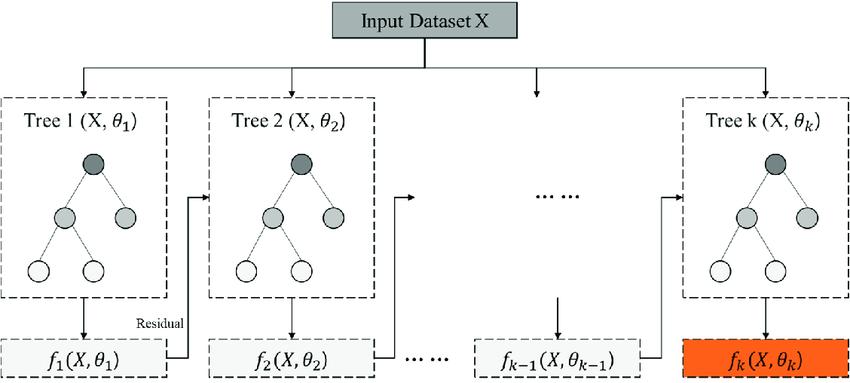
\includegraphics[width=10cm]{Figures/Background/XGBoost-model-process.png}
	\caption{Ejemplo de algoritmo \textit{XGBoost}}
	\label{XGBOOST_BACKGROUND}
\end{figure}


% \begin{figure}[H]
	%     \centering
	%     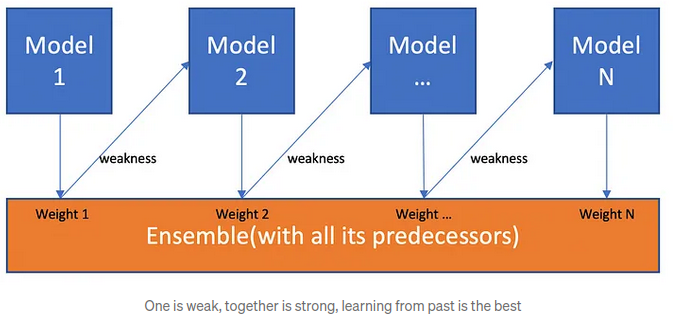
\includegraphics[width=14cm]{Figures/boosting_example.png}
	%     \caption{Alguna imagen así hecha por mi.}
	%     \label{BoostingExample}
	% \end{figure}

% [1] (https://towardsdatascience.com/boosting-algorithms-explained-d38f56ef3f30)

% [2] https://medium.com/geekculture/xgboost-versus-random-forest-898e42870f30


% https://towardsdatascience.com/best-practice-to-calculate-and-interpret-model-feature-importance-14f0e11ee660

% \section{Algoritmos Boosting}

% \textbf{Luis: jornada de reflexión sin redactar.} Yo creo que es que no hay boosting algorithms que ofrezcan la importancia de las características, creo  que de los pocos es el XGBoost. Hay que cercinoarse. No obstante, he visto esto:
% https://pubs.acs.org/doi/full/10.1021/ci0500379

\section{Algoritmos Genéticos}
% \underline{Explicación de los diferentes algoritmos genéticos que hay, formulas, descripcion, etc...}

% \textcolor{blue}{\textbf{Luis: Decir que son muy buenos para problemas de minimización (reducir coste y maximizar calidad, nos viene de lujo como entrada para la sección anterior)}}\\

Los algoritmos genéticos son métodos inspirados en la evolución biológica, que buscan optimizar soluciones a problemas matemáticos mediante la simulación de la evolución de una población de individuos que producen descendencia a lo largo de generaciones. Estos algoritmos han sido ampliamente utilizados en casos como la optimización del flujo de tráfico en la red para balancear la carga de los nodos \cite{5483775}, para analizar la capacidad de agua en el suelo mediante imágenes remotas \cite{PACHEPSKY1998213} o incluso para simular con el uso de autómatas distintas enfermedades como el \textit{COVID-19} \cite{GHOSH2020106692}. La principal fortaleza de estos algoritmos es que son métodos eficientes y seguros para llegar a soluciones aproximadas a la óptima ideal, reduciendo el coste computacional (en muchos casos exponencial), que supondría la búsqueda del óptimo global mediante métodos de combinación a lo largo de todo el espacio de búsqueda. Existen numerosos algoritmos genéticos conocidos, y muchos han sido aplicados a distintos contextos, tanto para problemas de objetivo único como a problemas multi-objetivo \cite{wang2020comparative}.

El funcionamiento de un algoritmo genético consta de una serie de etapas que son repetidas a lo largo de las sucesivas generaciones, concretamente \textit{inicialización, evaluación, selección, cruce, mutación y reemplazamiento}.

En la primera de ellas (\textit{inicialización}), se crea una población original de \textit{N} individuos aleatorios, donde cada uno de estos representa una posible solución al problema que se quiere optimizar (véase Figura \ref{GA_inicializacion}).

\begin{figure}[H]
	\centering
	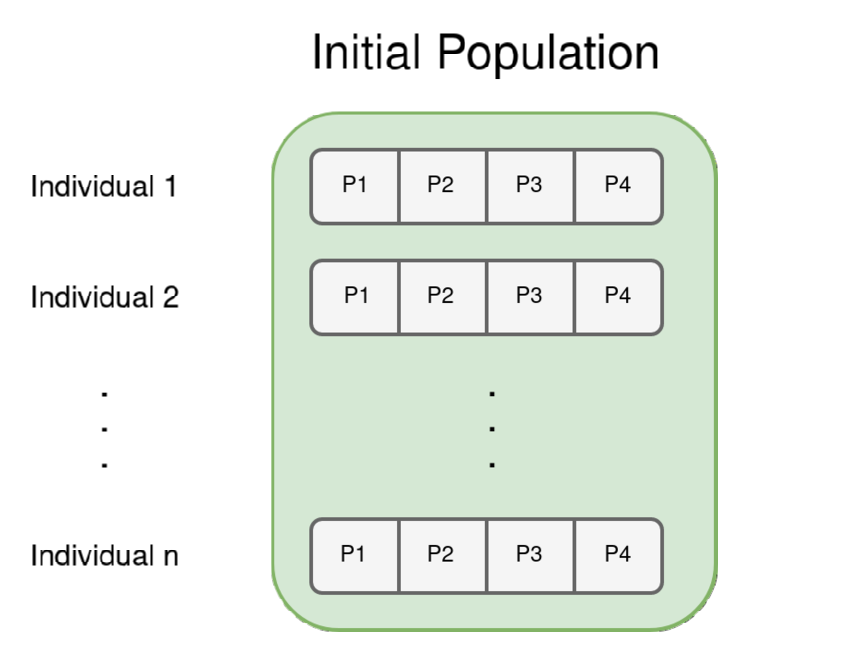
\includegraphics[width=6cm]{Figures/GA/inicializacion.png}
	\caption[Ejemplo de inicialización de individuos de algoritmo genético] {Ejemplo de inicialización de individuos de algoritmo genético. Este ejemplo consta de individuos compuestos por cuatro características}
	\label{GA_inicializacion}
\end{figure}


Estos individuos son evaluados mediante una función heurística, donde a cada uno se le asigna una puntuación de calidad en base a un criterio que mida el rendimiento que ofrece dicha solución al problema planteado (\textit{evaluación}), como se muestra en la Figura \ref{GA_selection}.


\begin{figure}[h]
	\centering
	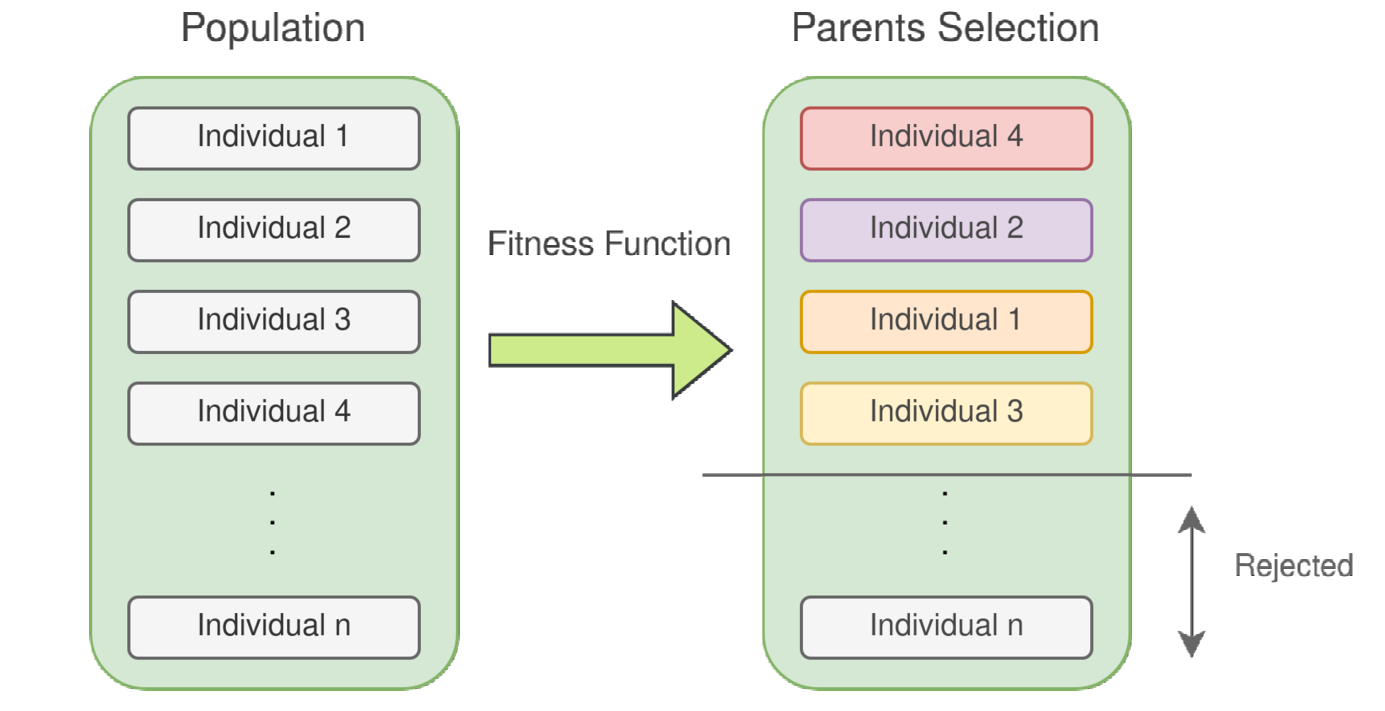
\includegraphics[width=8cm]{Figures/GA/selection.png}
	\caption[Ejemplo del proceso de selección de un algoritmo genético]{Ejemplo del proceso de selección de un algoritmo genético. En este ejemplo los cuatro mejores individuos de una generación son escogidos en base a su calidad en ofrecida por la función heurística (\textit{fitness function})}
	\label{GA_selection}
\end{figure}


Una vez se dispone de las puntuaciones de calidad, aquellos individuos que mejor se adapten al problema, es decir que mejor puntuación reciban, serán escogidos para dar lugar a descendencia (\textit{selección}). La información que contienen los \textit{M} mejores individuos es combinada entre sí (\textit{cruce}), simulando el intercambio de información producido en el intercambio genético en la naturaleza. Una vez se disponen de los nuevos individuos, estos pueden sufrir modificaciones aleatorias sobre su información resultante (\textit{mutación}), como se puede ver en la Figura \ref{GA_cruce_mutacion}.

\begin{figure}[h]
	\centering
	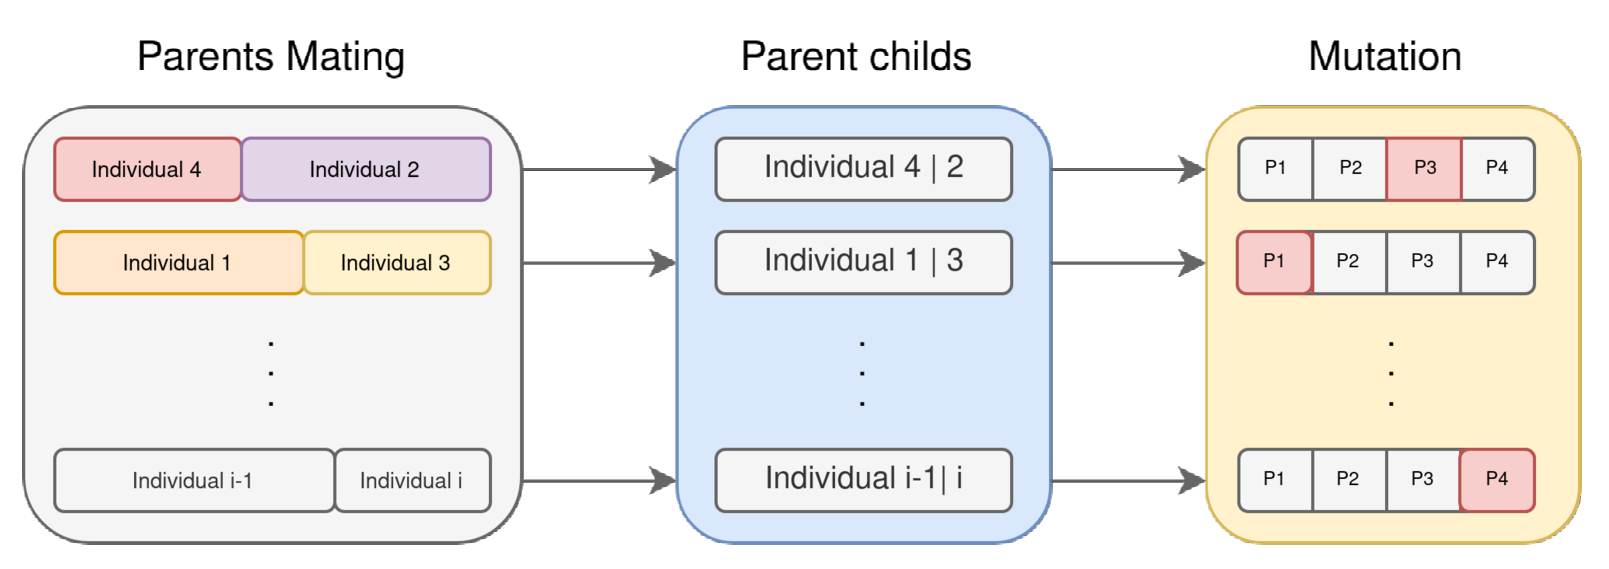
\includegraphics[width=10cm]{Figures/GA/cruce_mutacion.png}
	\caption[Ejemplo del proceso de cruce y mutación de un algoritmo genético] {Ejemplo del proceso de cruce y mutación de un algoritmo genético, donde se muta una característica de los individuos resultantes}
	\label{GA_cruce_mutacion}
\end{figure}

Como en cualquier población biológica, la combinación  de la misma información a lo largo de sucesivas generaciones provoca un estancamiento en la sociedad. La falta de diversidad en la población implica que no exista variabilidad en los individuos sucesores y por tanto que se tienda a explotar una zona del espacio de búsqueda provocando el riesgo de caer en un mínimo local del problema, es decir, una solución subóptima al problema respecto al mínimo global de la función buscado por estos algoritmos. Por este motivo es crucial introducir un componente aleatorio que pueda modificar la información de los individuos generados para tender a explorar este espacio de búsqueda. En este punto se evalúan los nuevos individuos y los \textit{M} miembros con peor puntuación de la población son eliminados, de esta forma la población en cada generación siempre constará de \textit{N} individuos. En caso de que existan individuos iguales en la población, estos son eliminados, lo que provoca que se integren en la población el mismo número de los que se han descartado. Estas etapas son repetidas a lo largo de varias generaciones hasta llegar a una condición de parada, tras la cual se seleccionará el individuo que mejor puntuación haya obtenido mediante la función heurística.

Cabe mencionar que dentro de la etapa de cruce, existen infinitas estrategias que se pueden aplicar para dar lugar al individuo descendiente. Por ejemplo, una de las más comunes suele consistir en dividir en dos a cada par de individuos que se reproducirán para generar su descendiente en base a composición de estas dos mitades. Otro método común, es seleccionar un punto aleatorio en cada proceso de descendencia del vector solución para dividir ambos progenitores, de tal forma que el individuo generado puede contener más información de un progenitor que de otro.


De esta forma, mediante la mejora continua de individuos a través de las generaciones, seleccionando los mejores y combinando su información entre sí, da lugar a una solución aproximada a la ideal a lo largo de las generaciones.

\section{Medidas de evaluación de una red neuronal}

En este apartado se presentan los indicadores de calidad utilizados para medir el rendimiento y generalización de los modelos expuestos en esta tesis. Uno de los componentes fundamentales en el desarrollo de modelos de inteligencia artificial es conocer la capacidad y calidad de los modelos ante la predicción de nuevas muestras que nunca ha visto durante su etapa de entrenamiento, tanto como para poder compararlos como para conocer en profundidad cómo se comportan los modelos ante nuevas situaciones.

Para evaluar los modelos, es común aplicar una fase de validación o de test, donde se utilizan los modelos para realizar predicciones contra muestras de las que se conoce su variable verdadera. De esta forma es posible comparar la calidad de los modelos respecto a muestras que nunca antes han visto y aplicar fórmulas y métricas que nos dan idea del rendimiento de los modelos. Para esto, es necesario introducir conceptos básicos que deben ser calculados para cada una de las clases que puede predecir el modelo.

\begin{enumerate}
	\item \textbf{True Positives (TP):} representan el número de muestras que han sido correctamente clasificadas por el modelo como positivas. Es decir, el modelo clasifica correctamente la muestra como la clase a la que pertenece.
	\item \textbf{True Negatives (TN):} representan el número de muestras que han sido correctamente clasificadas por el modelo como negativas. Es decir, el modelo
	\item \textbf{False Positives (FP):} representan el número de muestras que han sido incorrectamente clasificadas por el modelo como positivas. Es decir, el modelo ha clasificado una muestra que no pertenecía a esa clase como positiva.
	\item \textbf{False Negatives (FN):} representan el número de muestras que han sido incorrectamente clasificadas por el modelo como negativas. Es decir, el modelo ha clasificado una muestra positiva como negativa.
\end{enumerate}

En función del problema que nos encontremos, es posible que sea preferible un modelo que tienda a predecir con más facilidad futuras muestras a un tipo de clase respecto otra. Por ejemplo, es mejor predecir erróneamente que un accidente necesita asistencia (FP sobre la clase asistencia) y que luego no sea necesaria ninguna intervención, que predecir erróneamente uno que no necesita asistencia (FN sobre la clase No Asistencia). Este análisis del balance es posible evaluarlo gracias a los indicadores definidos anteriormente, no obstante, este tipo de decisiones son dependientes de la criticidad del problema que se quiere resolver.

Utilizando estos conceptos básicos es posible crear indicadores de calidad que ofrezcan más información para cada una de las clases predichas. En el estado del arte, se utilizan dos métricas comunes que pueden ser utilizadas para la composición de indicadores aún más complejos, estas métricas son calculadas para cada una de las posibles clases dentro del conjunto de datos.

La primera de ellas es la precisión (Precision), que mide el porcentaje de muestras clasificadas correctamente de una clase, respecto al total de muestras que existen de dicha clase en el conjunto de datos.

$$\text{Precision} = \frac{{\text{TP}}}{{\text{TP} + \text{FP}}}$$

Por otra parte, el recuerdo (\textit{Recall}) representa la proporción de elementos de una clase que el modelo identifica correctamente como esa clase.

$$\text{Recall} = \frac{{\text{TP}}}{{\text{TP} + \text{FN}}}$$

Existe otra métrica que combina los dos indicadores anteriores, considerando la precisión que tiene el modelo a la hora de predecir muestras como una clase y cuántos de los casos positivos fueron captados por el modelo (recuerdo), de tal forma que para cada cada una de las clases se pueda obtener una evaluación individual, siendo más sencillo en análisis sobre esto. 

$$\text{F1 score} = 2 \times \frac{{\text{precision} \times \text{recall}}}{{\text{precision} + \text{recall}}}$$


%\textcolor{red}{AQUI estaría interesante poner un minipárrafo destacando lo maravillosa que es esta medida, para que se suele usar, y tal. Más que nada porque luego la usamos para resaltar los buenos resultados obtenidos.}

%\textcolor{orange}{\textbf{Luis: } Hecho}

La métrica F1-Score es particularmente útil en problemas de clasificación binaria, sobre todo cuando existe un desbalanceo en las clases. Particularmente en estos casos, este indicador muestra información muy relevante en comparación a otras por sí solas, ya que toma en cuenta la combinación tanto de los falsos positivos como de los falsos negativos. Debido a la visión general del rendimiento de los modelos que ofrece en este tipo de casos, será la métrica definida para la evaluación de los modelos sen esta tesis.


